
\section{Background and Related Work} 
\label{sec:related} 
% 
\ac{DNS} owes its precision to the lack of any modeling assumptions and the high
resolution of the simulation grid. Important \ac{DNS} applications are presented in
\cite{Hilbert2004}. Most of the simulated variables are related to chemistry.
Simulations of practically relevant reactions are complex and involve tens or
even hundreds of chemical variables. Due to both the high resolution and the
large number of variables, a simulation run produces terabytes of raw data.
These amounts cannot be stored or transferred efficiently, prompting the need of
methods for either analyzing in-situ or reducing them.

%------
Analysis of such raw data is usually done in a post-processing step: Bremer et
al.~\cite{Bremer2009} present a framework for exploring burning clusters in
combustion simulations by generating a level-set-based topological hierarchy;
Akiba et al.~\cite{Akiba2007} display multiple superimposed isosurfaces and
direct volume renderings. Further post-processing methods are described in Zistl
et al.~\cite{Zistl2009}. All approaches rely on the raw data being available
after the simulation, thus ignoring problem~\ref{i:size}. If the raw data is too
large to be stored completely, post-processing can not be performed at all.

% However, due to their large size, only few time steps are stored,
% the data is downsampled to a lower spatial resolution, or both. This means,
% standard post-processing methods become ineffective, since the data they are
% supposed to analyze is simply discarded.

To address this issue, in-situ visualization methods have been developed.
They process and render simulation data while being produced, operating in
parallel with the simulation on the same supercomputer. 
%
% This provides
% significant challenges. Many supercomputers have limited graphics hardware, and
% communication in these massively parallel machines is the main bottleneck. The
% rendering therefore has to use the same data decomposition as the simulation,
% which is not optimized for visualization. 
%
This type of in-situ visualization is discussed in \cite{Ma2009}, while
\cite{Yu2010} describes a specific renderer for volume and particle data. These
methods provide a superior way of monitoring the simulation progress. However,
they do not offer a solution to problem~\ref{i:analyze}. Since they only output
rendered images, more detailed analysis still has to be performed on the huge
original data sets.

% While these methods are good at efficiently
% creating renderings of all time steps, thus providing a superior way of progress
% monitoring, they are less flexible in the way the data can be analyzed.
% Obviously, a single volume rendering can seldom replace a detailed analysis.
% More complex analysis steps also have to operate parallel to the simulation,
% suffering from the same problems as in-situ rendering.

One way to achieve both flexibility and storage-efficiency is to compress the
data before storing it. The compressed data can then be decoded and analyzed
with any method. Numerous compression methods exist, but few are well-suited for
\ac{DNS} data. The \ac{3D}-\acs{SPIHT} (\acl{SPIHT}\acused{SPIHT})
algorithm~\cite{Kim2000} uses a global wavelet transform to compress volume
data. A blockwise wavelet-based approach tailored to visualization applications
is proposed in \cite{Nguyen2001}. Fout et al.~\cite{Fout2005} describe a vector
quantization approach designed for fast decompression using graphics hardware,
enabling fast volume rendering of compressed data. These approaches provide
high-accuracy, lossy compression for general volume data. However, they do not
take into account the special requirements of analyzing combustion data, thus
ignoring problems~\ref{i:analyze} and~\ref{i:visualize}.
%
% @dirk: hier feature preserving nennen

%----Hier überleitung 
%
Our work focuses on \ac{DNS} of premixed combustion: generally, a mixture of chemical
species react and form products, as described in \cite{Fru2011}. Reactions do
not happen simultaneously in the whole mixture. Rather, flame fronts spread out
from spots of ignition. Reactions only occur in these thin zones, consuming fuel
and oxidizer and leaving hot products behind. During the reaction, intermediate,
unstable compounds form, which only occur in the flame front and quickly react
with other compounds to form stable end products. Outside of the flame front,
and therefore in most of the simulated volume, concentrations of chemical
variables are close to constant. Inside, these variables vary most rapidly along
the shortest path across the front, and their values are therefore highly
correlated.

To simplify the investigation of the flame shape, a flame surface representing
the flame front is commonly defined as the surface separating burned and unburnt
gases. It is contained in the flame front and its surface normal is aligned with
the gradients of the scalar variables.
%
%Since the reaction zone is not infinitely thin, the location of this surface is not uniquely
%defined. Different definitions will however always be contained in the reaction
%zone and be almost orthogonal to the gradient vectors of the simulation variables.
%
Interaction with turbulence causes this flame surface to become wrinkled,
producing areas of high curvature. The flame surface can be defined in different
ways based on the scalar fields of the simulation. Often it is defined as an
isosurface, surface of maximum value, or surface of steepest slope. These
feature surfaces are similar, but their differences give meaningful insights
into the combustion process. Our sparse representation directly captures these
feature surfaces and enables their analysis and visualization (see
\cref{fig_contourmeshvis}).

\begin{figure}[t]
    \setlength\figurewidth\textwidth
    \centering
    \begin{tikzpicture}[
    label/.style={anchor=north west, font=\small},
]
\newlength\imgwidth
\setlength\imgwidth{0.2\figurewidth - 1.6mm}
\matrix (m) [
    matrix of nodes,
    column sep=2mm,
    row sep=2mm,
    inner sep=0,
    outer sep=0
]{
    
\includegraphics[width=\imgwidth]{images/CO_orig_rdoryl_s.png} &
    
\includegraphics[width=\imgwidth]{images/H2_orig_rdoryl_s.png} &
    
\includegraphics[width=\imgwidth]{images/O2_orig_rdoryl_s.png} &
    
\includegraphics[width=\imgwidth]{images/T_orig_rdoryl_s.png} &
    
\includegraphics[width=\imgwidth]{images/CO2_orig_rdoryl_s.png} \\
    
\includegraphics[width=\imgwidth]{images/H2O_orig_rdoryl_s.png} &
    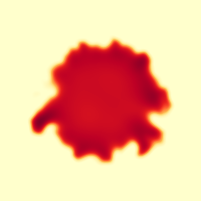
\includegraphics[width=\imgwidth]{images/OH_orig_rdoryl_s.png} &
    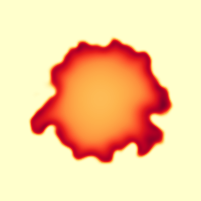
\includegraphics[width=\imgwidth]{images/O_orig_rdoryl_s.png} &
    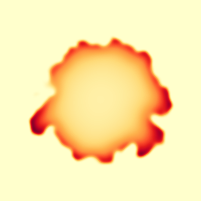
\includegraphics[width=\imgwidth]{images/H_orig_rdoryl_s.png} &
    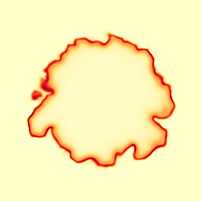
\includegraphics[width=\imgwidth]{images/H2O2_orig_rdoryl_s.png} \\
    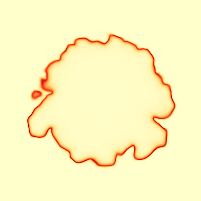
\includegraphics[width=\imgwidth]{images/HO2_orig_rdoryl_s.png} &
    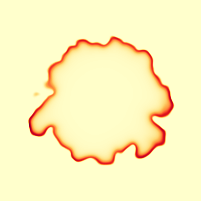
\includegraphics[width=\imgwidth]{images/HCO_orig_rdoryl_s.png} &
    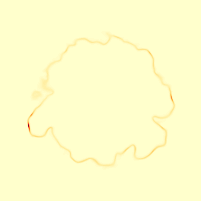
\includegraphics[width=\imgwidth]{images/CH2O_orig_rdoryl_s.png} &
    \begin{tikzpicture}
        \draw[draw=none] (0, 0) rectangle (\imgwidth, \imgwidth);
        \node[
            draw=black,
            anchor=south west,
            thin,
            inner sep=0.05mm
        ] (cmap) at (0, 0) {%
            \rotatebox{-90}{%
                
\includegraphics[height=0.25cm, width=\imgwidth]{figures/rdoryl.png}%
            }
        };
        \node[
            anchor=north west,
            font=\small,
            inner sep=0,
            xshift=1mm
        ] at (cmap.north east) {max};
        \node[
            anchor=south west,
            font=\small,
            inner sep=0,
            xshift=1mm
        ] at (cmap.south east) {min};
    \end{tikzpicture}&
    \tikz{\draw[draw=none] (0, 0) rectangle (\imgwidth, \imgwidth);} \\
};

\node[label, white] at (m-1-1.north west) {\ce{CO}};
\node[label, white] at (m-1-2.north west) {\ce{H2}};
\node[label, white] at (m-1-3.north west) {\ce{O2}};
\node[label] at (m-1-4.north west) {\ce{T}};
\node[label] at (m-1-5.north west) {\ce{CO2}};
\node[label] at (m-2-1.north west) {\ce{H2O}};
\node[label] at (m-2-2.north west) {\ce{OH}};
\node[label] at (m-2-3.north west) {\ce{O}};
\node[label] at (m-2-4.north west) {\ce{H}};
\node[label] at (m-2-5.north west) {\ce{H2O2}};
\node[label] at (m-3-1.north west) {\ce{HO2}};
\node[label] at (m-3-2.north west) {\ce{HCO}};
\node[label] at (m-3-3.north west) {\ce{CH2O}};


\end{tikzpicture}
    \vspace*{-5mm}
    \caption{Slices of simulation variables of a premixed turbulent syngas flame}
    \label{fig:sim_vars}
\end{figure}

% In this work, we describe a space-saving sparse representation for \ac{DNS} data of
% premixed combustion which captures the characteristics of the scalar fields
% and can directly be used for visualizing their differences. In the following, we
% describe the transformation of the raw data into the sparse form, as well as the
% reconstruction of the original scalar fields from this form. We then present a
% visualization approach for comparing the relations between the scalar fields
% over time based on this representation. We demonstrate the effectiveness of our
% approach on multiple real datasets.

% In this work, we describe a novel feature-preserving compression approach
% providing high compression ratios while maintaining good accuracy.
% Our approach explicitly identifies data features, which can later be visualized
% without the need for decompression. Subsequently, we describe the compression,
% and afterwards the visualization approach for \ac{DNS} data.
